\documentclass[12pt, a4paper]{book}

\usepackage[T1]{fontenc}
\usepackage[utf8]{inputenc}
\usepackage[charter, cal=cmcal]{mathdesign}
\usepackage[scaled=0.92]{helvet}
\usepackage{geometry}
\geometry{a4paper, top=30mm, bottom=30mm, inner=32mm, outer=25mm, marginparwidth=18mm}

\usepackage{amsmath, amsthm}
\usepackage[version=4]{mhchem}
\usepackage{graphicx}
\usepackage{xcolor}
\usepackage{tikz}
\usetikzlibrary{arrows.meta, shapes.geometric, positioning, calc, backgrounds}
\usepackage{pgfplots}
\pgfplotsset{compat=1.18}
\usepackage{tcolorbox}
\tcbuselibrary{skins, breakable, theorems}
\usepackage{titlesec}
\usepackage{fancyhdr}
\usepackage{enumitem}
\usepackage{booktabs}
\usepackage{array}
\usepackage{parskip}
\usepackage{siunitx}
\usepackage[colorlinks=true, linkcolor=BrickRed,
            urlcolor=NavyBlue, citecolor=ForestGreen]{hyperref}

% ── Colours (Journey 5 — forest green / amber) ────────────────────────────────
\definecolor{JourneyColor}{HTML}{065F46}
\definecolor{ModuleColor}{HTML}{059669}
\definecolor{PuzzleColor}{HTML}{B45309}
\definecolor{DiscoveryColor}{HTML}{D97706}
\definecolor{WarningColor}{HTML}{991B1B}
\definecolor{ProblemColor}{HTML}{6B21A8}
\definecolor{ReflectColor}{HTML}{0D9488}
\definecolor{HistoryColor}{HTML}{78350F}

% ── Boxes ─────────────────────────────────────────────────────────────────────
\newtcolorbox{puzzlebox}[1][]{enhanced,breakable,
  colback=PuzzleColor!6,colframe=PuzzleColor,fonttitle=\bfseries\sffamily,
  title={The Puzzle},attach boxed title to top left={yshift=-2mm,xshift=6mm},
  boxed title style={colback=PuzzleColor},borderline west={3pt}{0pt}{PuzzleColor},#1}

\newtcolorbox{discoverybox}[1][]{enhanced,breakable,
  colback=DiscoveryColor!8,colframe=DiscoveryColor,fonttitle=\bfseries\sffamily,
  title={Discovery},attach boxed title to top left={yshift=-2mm,xshift=6mm},
  boxed title style={colback=DiscoveryColor},borderline west={3pt}{0pt}{DiscoveryColor},#1}

\newtcolorbox{problembox}[1][]{enhanced,breakable,
  colback=ProblemColor!5,colframe=ProblemColor,fonttitle=\bfseries\sffamily,
  title={Problems},attach boxed title to top left={yshift=-2mm,xshift=6mm},
  boxed title style={colback=ProblemColor},borderline west={3pt}{0pt}{ProblemColor},#1}

\newtcolorbox{deepbox}[1][]{enhanced,breakable,
  colback=JourneyColor!5,colframe=JourneyColor,fonttitle=\bfseries\sffamily,
  title={Deep Problems},attach boxed title to top left={yshift=-2mm,xshift=6mm},
  boxed title style={colback=JourneyColor},borderline west={4pt}{0pt}{JourneyColor},#1}

\newtcolorbox{historybox}[1][]{enhanced,breakable,
  colback=HistoryColor!7,colframe=HistoryColor!60,fonttitle=\bfseries\sffamily\small,
  title={Historical Note},attach boxed title to top left={yshift=-2mm,xshift=6mm},
  boxed title style={colback=HistoryColor!80},#1}

\newtcolorbox{reflectionbox}[1][]{enhanced,breakable,
  colback=ReflectColor!6,colframe=ReflectColor,fonttitle=\bfseries\sffamily,
  title={Reflection},attach boxed title to top left={yshift=-2mm,xshift=6mm},
  boxed title style={colback=ReflectColor},borderline west={3pt}{0pt}{ReflectColor},#1}

\newtcolorbox{namedconcept}[2][]{enhanced,
  colback=ModuleColor!6,colframe=ModuleColor,fonttitle=\bfseries\sffamily\large,
  title={#2},attach boxed title to top left={yshift=-2mm,xshift=6mm},
  boxed title style={colback=ModuleColor},#1}

% ── Section formatting ────────────────────────────────────────────────────────
\titleformat{\chapter}[display]
  {\normalfont\sffamily\huge\bfseries\color{JourneyColor}}
  {\textcolor{JourneyColor!60}{\chaptertitlename\ \thechapter}}{10pt}{\Huge}
  [\vspace{2pt}\textcolor{JourneyColor}{\titlerule[1.5pt]}]
\titleformat{\section}
  {\normalfont\sffamily\Large\bfseries\color{ModuleColor}}
  {\thesection}{1em}{}[\textcolor{ModuleColor!40}{\titlerule[0.6pt]}]
\titleformat{\subsection}
  {\normalfont\sffamily\large\bfseries\color{JourneyColor!80}}{\thesubsection}{1em}{}
\titleformat{\subsubsection}
  {\normalfont\sffamily\normalsize\bfseries}{\thesubsubsection}{1em}{}

\pagestyle{fancy}
\fancyhf{}
\fancyhead[LE]{\small\sffamily\textcolor{JourneyColor}{\leftmark}}
\fancyhead[RO]{\small\sffamily\textcolor{ModuleColor}{\rightmark}}
\fancyfoot[C]{\small\thepage}
\renewcommand{\headrulewidth}{0.4pt}

\newcommand{\newterm}[1]{\textit{\textcolor{DiscoveryColor}{#1}}}
\newcommand{\important}[1]{\textcolor{ModuleColor}{\textbf{#1}}}

\begin{document}

\setcounter{chapter}{4}
\chapter[Journey 5 --- Chemical Kinetics and Dynamics]
        {Journey Five\\[8pt]
         \textcolor{ModuleColor}{\large Chemical Kinetics and Dynamics}}
\setcounter{section}{1}

\section{Module 5.2 --- Temperature Dependences and Activation Energies}
\label{sec:mod5.2}

\subsection*{Motivation}

We discovered in Module 5.1 how chemical rates evolve as a function of concentrations.
However, if you raise the temperature of a reaction mixture, the speed changes dramatically.
For many common reactions at room temperature, a tiny temperature increase of only \SI{10}{\degree C} causes the reaction rate to *double*.

If temperature is merely a measure of average kinetic energy ($E_k \propto T$), a \SI{10}{\degree C} increase (from \SI{298}{K} to \SI{308}{K}) represents a microscopic kinetic energy increase of only $\sim 3\%$.
Yet the reaction rate increases by $100\%$.
Why is the rate of chemical reactions so exponentially sensitive to temperature?
This module explores collision theory and transition state theory to discover the activation barriers that molecules must climb to transform.

\subsection{Collision Theory and the Energetic Barrier}

For a chemical reaction to occur, reactant molecules must collide in space. But not all collisions are successful.

\begin{puzzlebox}
\textbf{The Kinetic Threshold.}

Suppose we have a gas-phase reaction:
\[
  \ce{A(g) + B(g) -> C(g) + D(g)}.
\]
\begin{enumerate}[label=(\alph*), leftmargin=*]
  \item Classically, the average speed of gas molecules scales as $v_{\text{avg}} \propto \sqrt{T}$. If the reaction rate depended only on the frequency of physical collisions, how would the rate constant $k$ scale with temperature? Calculate the percentage increase in collision frequency when temperature rises from \SI{298}{K} to \SI{308}{K}.
  \item In reality, only a tiny fraction of collisions results in a reaction. Why is this? If we collide two billiard balls covered in wet paint, they only transfer paint if they touch. In chemistry, what must happen to the chemical bonds during a collision?
  \item Svante Arrhenius proposed that molecules must possess a minimum kinetic energy, the **activation energy** $E_a$, to react during a collision.
  Using the Maxwell-Boltzmann distribution you explored in Physics Journey 6 Module 1, the fraction $f$ of molecules with kinetic energy greater than $E_a$ is proportional to:
  \[
    f \;\propto\; e^{-\frac{E_a}{RT}},
  \]
  where $R \approx 8.314$ J$\cdot$mol$^{-1}$K$^{-1}$ is the gas constant.
  Compute the value of $f$ for $E_a = 50$ kJ/mol at $T = 298$ K and $T = 308$ K. Does this fraction double?
\end{enumerate}
\end{puzzlebox}

\subsection{The Arrhenius Equation}

We combine collision frequency, orientation factors, and the thermal energy fraction into a single rate relation.

\begin{explobox}
For a collision to result in a reaction, the molecules must satisfy two criteria:
1. **Energy:** They must collide with kinetic energy $E \ge E_a$.
2. **Orientation:** They must collide in the correct spatial alignment (the steric factor $p$).

This yields the **Arrhenius Equation**:
\[
  k \;= \; A e^{-\frac{E_a}{RT}},
\]
where $A$ is the **pre-exponential factor** (or frequency factor), representing the rate of collisions with the correct orientation.
\begin{enumerate}[label=(\alph*), leftmargin=*]
  \item Plot $k$ as a function of temperature $T$. Why does the rate constant grow exponentially?
  \item What is the physical meaning of the limit of $k$ as $T \to \infty$?
  \item Show that we can linearize the Arrhenius equation by taking the natural logarithm:
  \[
    \ln k \;=\; \ln A - \frac{E_a}{R}\left(\frac{1}{T}\right).
  \]
  If we plot $\ln k$ versus $1/T$, why does this yield a straight line? What represents the slope? What represents the $y$-intercept?
  \item Show that by measuring the rate constant at two different temperatures, $T_1$ and $T_2$, we can calculate the activation energy $E_a$ without knowing $A$:
  \[
    \ln\left( \frac{k_2}{k_1} \right) \;=\; -\frac{E_a}{R}\left( \frac{1}{T_2} - \frac{1}{T_1} \right).
  \]
\end{enumerate}
\end{explobox}

\subsection{Transition State Theory}

We model the path of the reaction over an energy barrier.

\begin{explobox}
During a collision, the reactants deform, bonds stretch, and they briefly form a highly unstable, high-energy configuration called the **transition state** or **activated complex** ($\ce{X^\ddagger}$).
\begin{center}
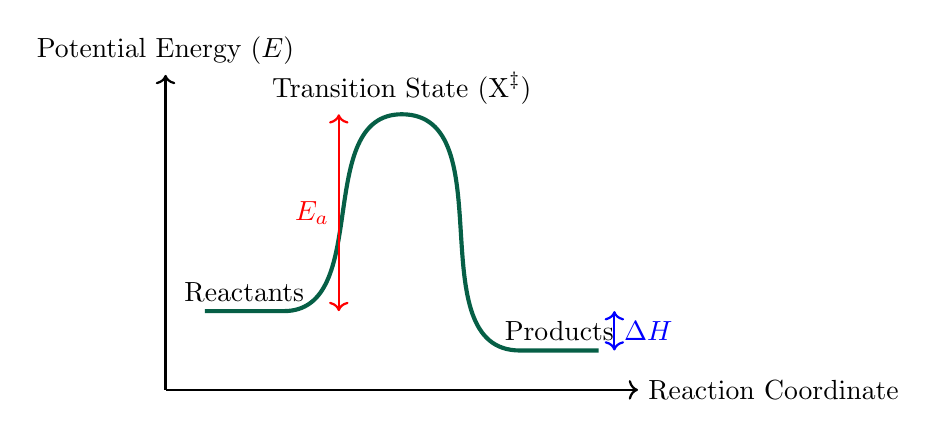
\begin{tikzpicture}[scale=1.0]
  % Reaction coordinate diagram
  \draw[->, thick] (0,0) -- (6,0) node[right] {Reaction Coordinate};
  \draw[->, thick] (0,0) -- (0,4) node[above] {Potential Energy ($E$)};
  
  % Energy curve
  \draw[line width=1.5pt, JourneyColor] (0.5,1) -- (1.5,1) 
    to[out=0,in=180] (3,3.5) 
    to[out=0,in=180] (4.5,0.5) -- (5.5,0.5);
    
  % Labels
  \node[above] at (1,1) {Reactants};
  \node[above] at (5,0.5) {Products};
  \node[above] at (3,3.5) {Transition State ($\ce{X^\ddagger}$)};
  
  % Activation energy arrow
  \draw[<->, red, thick] (2.2,1) -- (2.2,3.5);
  \node[left, red] at (2.2,2.25) {$E_a$};
  
  % Delta H arrow
  \draw[<->, blue, thick] (5.7,1) -- (5.7,0.5);
  \node[right, blue] at (5.7,0.75) {$\Delta H$};
\end{tikzpicture}
\end{center}
\begin{enumerate}[label=(\alph*), leftmargin=*]
  \item Let a reaction be exothermic ($\Delta H < 0$), as shown in the diagram. Explain why even an exothermic reaction requires an input of activation energy to proceed.
  \item The transition state corresponds to a local maximum along the reaction coordinate. Why can we never isolate the activated complex in a bottle? (What is its lifetime compared to stable molecules?)
\end{enumerate}
\end{explobox}

\newpage

% ─── Section: Discovery ──────────────────────────────────────────────────────
\section{Part 3 --- Discovery}

\begin{discoverybox}
\textbf{What have we built?}

\textbf{First.} The exponential temperature dependence of chemical rates arises because only a tiny fraction of molecules possess enough thermal energy to climb the activation barrier.

\textbf{Second.} The Arrhenius equation $k = A e^{-E_a/RT}$ relates the rate constant to temperature. The frequency factor $A$ represents the rate of properly oriented collisions, while $E_a$ is the activation threshold.

\textbf{Third.} Linearizing the Arrhenius equation yields $\ln k = \ln A - \frac{E_a}{R}(\frac{1}{T})$. Plotting $\ln k$ versus $1/T$ (an Arrhenius plot) is the standard experimental method to extract $E_a$ (from the slope) and $A$ (from the intercept).

\textbf{Fourth.} The transition state is a transient, high-energy configuration at the peak of the potential energy barrier. The activation energy is the energy required to deform the reactants into this activated complex.
\end{discoverybox}

\newpage

% ─── Section: Naming Concepts ────────────────────────────────────────────────
\section{Part 4 --- What This Is Called}

\begin{namedconcept}{Temperature kinetics parameters}
* **Activation Energy ($E_a$):** The minimum kinetic energy colliding molecules must possess to initiate a chemical reaction.
* **Pre-exponential Factor ($A$):** The frequency factor representing the total collision frequency times the probability of correct orientation (steric factor $p$).
* **Activated Complex (Transition State):** The transient configuration at the potential energy maximum along the reaction path.
* **Arrhenius Plot:** A graph of $\ln k$ versus $1/T$. The slope is $-E_a/R$, and the $y$-intercept is $\ln A$.
\end{namedconcept}

\newpage

% ─── Section: Solved Exercises ───────────────────────────────────────────────
\section{Part 5 --- Solved Exercises}

\begin{problembox}
\begin{enumerate}[label=\textbf{E\arabic*.}]
  \item \textbf{Calculating Activation Energy from Two Rates.}
  
        The rate constant of a reaction doubles when the temperature is raised from \SI{298}{K} to \SI{308}{K}. Calculate the activation energy $E_a$ of this reaction.
        
        \textbf{Solution:}
        We are given:
        \[
          T_1 \;=\; 298 \text{ K}, \qquad T_2 \;=\; 308 \text{ K}, \qquad \frac{k_2}{k_1} \;=\; 2.
        \]
        We use the two-temperature Arrhenius relation:
        \[
          \ln\left( \frac{k_2}{k_1} \right) \;=\; -\frac{E_a}{R}\left( \frac{1}{T_2} - \frac{1}{T_1} \right).
        \]
        Substitute the known values:
        \[
          \ln(2) \;=\; -\frac{E_a}{8.314}\left( \frac{1}{308} - \frac{1}{298} \right).
        \]
        Calculate the difference inside the parenthesis:
        \[
          \frac{1}{308} - \frac{1}{298} \;=\; 0.003247 - 0.003356 \;=\; -1.09 \times 10^{-4} \text{ K}^{-1}.
        \]
        Substitute this back and evaluate $\ln(2) \approx 0.693$:
        \[
          0.693 \;=\; -\frac{E_a}{8.314} \left( -1.09 \times 10^{-4} \right) \implies 0.693 \;=\; E_a \left( 1.31 \times 10^{-5} \right).
        \]
        Solve for $E_a$:
        \[
          E_a \;=\; \frac{0.693}{1.31 \times 10^{-5}} \;=\; 5.29 \times 10^4 \text{ J/mol} \;=\; 52.9 \text{ kJ/mol}.
        \]
        Thus, the activation energy of the reaction is \SI{52.9}{kJ/mol}.
        
  \item \textbf{Arrhenius Slope and Intercept Verification.}
  
        Prove that the slope of an Arrhenius plot ($\ln k$ vs. $1/T$) is $-E_a/R$, and show how to determine the pre-exponential factor $A$ from the graph.
        
        \textbf{Solution:}
        Let $y = \ln k$ and $x = 1/T$. The legalized Arrhenius equation is:
        \[
          \ln k \;=\; -\frac{E_a}{R}\left(\frac{1}{T}\right) + \ln A.
        \]
        This has the standard linear form:
        \[
          y \;=\; m x + c,
        \]
        where:
        * The independent variable is $x = 1/T$.
        * The dependent variable is $y = \ln k$.
        * The slope is $m = -E_a/R$.
        * The $y$-intercept is $c = \ln A$.
        
        To find $E_a$ from a plotted line, we measure the slope $m = \frac{\Delta \ln k}{\Delta (1/T)}$, and calculate:
        \[
          E_a \;=\; -R \cdot m.
        \]
        To find $A$, we locate the $y$-intercept $c$ (the value of $\ln k$ when $1/T = 0$, representing infinite temperature), and calculate:
        \[
          A \;=\; e^c.
        \]
        This completes the proof.
\end{enumerate}
\end{problembox}

\newpage

% ─── Section: Problems ───────────────────────────────────────────────────────
\section{Part 6 --- Problems}

\begin{problembox}
\begin{enumerate}[label=\textbf{P\arabic*.}]
  \item \textbf{Cricket Chirping and Biology.}
  
        The chirping frequency of snowy tree crickets is exponentially temperature-dependent (Dolbear's Law). The physiological rate-limiting reaction governing the chirping fits the Arrhenius relation: $f \approx A e^{-E_a/RT}$.
        \begin{enumerate}[label=(\alph*)]
          \item A cricket is observed to chirp 100 times per minute at \SI{15}{\degree C} (\SI{288}{K}), and 200 times per minute at \SI{25}{\degree C} (\SI{298}{K}). Calculate the activation energy $E_a$ of this biological reaction.
          \item What is the chirping frequency you would predict at \SI{35}{\degree C}?
        \end{enumerate}

  \item \textbf{Steric Factors and Gas collisions.}
  
        For the gas-phase reaction of nitric oxide and ozone:
        \[
          \ce{NO(g) + O3(g) -> NO2(g) + O2(g)}
        \]
        the activation energy is $E_a = 10.0$ kJ/mol. The experimentally measured pre-exponential factor is $A = 2.0 \times 10^9$ M$^{-1}$s$^{-1}$ at \SI{300}{K}.
        Using collision theory, the calculated physical collision rate of the two spheres is $Z = 1.0 \times 10^{11}$ M$^{-1}$s$^{-1}$.
        \begin{enumerate}[label=(\alph*)]
          \item Calculate the steric factor $p = A/Z$.
          \item Explain what this value of $p$ suggests about the orientation requirements of the collision. Draw a sketch of a successful collision versus an unsuccessful one.
        \end{enumerate}
\end{enumerate}
\end{problembox}

\newpage

% ─── Section: Deep Problems ──────────────────────────────────────────────────
\section{Part 7 --- Deep Problems}

\begin{deepbox}
\begin{enumerate}[label=\textbf{D\arabic*.}]
  \item \textbf{Transition State Theory and the Eyring Equation.}
  
        Henry Eyring and Michael Polanyi developed a thermodynamic model of transition states. They proposed that the reactants exist in a quasi-equilibrium with the transition state complex $\ce{X^\ddagger}$:
        \[
          \ce{A + B <=> X^\ddagger -> Products}.
        \]
        The rate constant is given by the **Eyring Equation**:
        \[
          k \;=\; \kappa \frac{k_B T}{h} e^{-\frac{\Delta G^\ddagger}{RT}},
        \]
        where $\kappa \le 1$ is the transmission coefficient, $h$ is Planck's constant, and $\Delta G^\ddagger = \Delta H^\ddagger - T \Delta S^\ddagger$ is the activation free energy.
        \begin{enumerate}[label=(\alph*)]
          \item Show that the Eyring equation can be rewritten as:
          \[
            k \;=\; \left( \kappa \frac{k_B T}{h} e^{\frac{\Delta S^\ddagger}{R}} \right) e^{-\frac{\Delta H^\ddagger}{RT}}.
          \]
          \item Compare this to the Arrhenius equation $k = A e^{-E_a/RT}$. Identify the activation enthalpy $\Delta H^\ddagger$ and activation entropy $\Delta S^\ddagger$ in terms of $E_a$ and $A$.
          \item If a reaction requires a highly ordered transition state, what is the sign of the activation entropy $\Delta S^\ddagger$? How does this affect the frequency factor $A$?
        \end{enumerate}

  \item \textbf{The Kinetic Isotope Effect.}
  
        In Physics Journey 6 Module 3, you proved that the ground-state zero-point vibrational energy of a harmonic oscillator is $E_0 = \frac{1}{2}\hbar\omega$, where $\omega = \sqrt{k_f/\mu}$ ($k_f$ is the bond force constant, and $\mu$ is the reduced mass of the two atoms).
        Replacing hydrogen ($\ce{^1H}$) with deuterium ($\ce{^2H}$) in a carbon-hydrogen bond ($\ce{C-H}$) slows down the rate of cleavage reactions significantly (often by a factor of 7).
        \begin{enumerate}[label=(\alph*)]
          \item Calculate the reduced mass ratio $\mu_{\ce{C-D}}/\mu_{\ce{C-H}}$, assuming carbon has mass 12. Show that the zero-point energy of the $\ce{C-D}$ bond is lower than that of the $\ce{C-H}$ bond.
          \item Assuming the transition state has the carbon-hydrogen bond completely broken (vibrational energy is zero), sketch the potential energy curves for the cleavage of $\ce{C-H}$ and $\ce{C-D}$ bonds.
          \item Show why the difference in zero-point energies implies that the activation energy for cleavage of the $\ce{C-D}$ bond is larger than that of the $\ce{C-H}$ bond, explaining the **Kinetic Isotope Effect**.
        \end{enumerate}
\end{enumerate}
\end{deepbox}

\newpage

% ─── Section: Reflection ─────────────────────────────────────────────────────
\section{Part 8 --- Reflection}

\begin{reflectionbox}
\textbf{Conceptual Reflection}

Consider the following questions:
\begin{enumerate}
  \item **On the Steric Factor:** The reaction steric factor $p$ can be as small as $10^{-6}$ for complex proteins. What does this tell you about the efficiency of simple molecular collisions? How do biological enzymes overcome this orientation barrier?
  \item **On Free Energy:** The Eyring equation expresses the rate constant in terms of activation free energy $\Delta G^\ddagger = \Delta H^\ddagger - T\Delta S^\ddagger$. Why does this show that reaction speed is governed not just by energy ($\Delta H^\ddagger$), but also by configuration space entropy ($\Delta S^\ddagger$)?
  \item **On Isotope Effects:** The kinetic isotope effect is a direct macroscopic measurement of quantum zero-point energy. If zero-point energy did not exist ($\hbar = 0$), would replacing hydrogen with deuterium affect the speed of chemical reactions?
\end{enumerate}
\end{reflectionbox}

\medskip
\noindent\textbf{Looking ahead.}
Module~5.3 introduces **Reaction Mechanisms**. We will use our rate laws and activation energies to study how complex reactions are built from elementary steps. We will discover the rate-determining step and apply the steady-state approximation to model chemical kinetics.

\vspace{1.4cm}
\begin{center}
{\color{JourneyColor}\rule{0.5\linewidth}{0.8pt}}\\[6pt]
{\small\color{JourneyColor}\textit{End of Journey 5, Module 5.2 --- Temperature Dependences and Activation Energies}}\\[4pt]
{\small\color{JourneyColor}Continue to: \textbf{Module 5.3 --- Reaction Mechanisms}}\\[6pt]
{\color{JourneyColor}\rule{0.5\linewidth}{0.8pt}}
\end{center}

\end{document}
